\documentclass[a4,12pt]{article}
\usepackage[utf8]{inputenc} % para acentos y eñes
\usepackage[spanish]{babel}
\usepackage{verbatim} % para comentarios multilinea
\usepackage{graphicx} % para imagenes
\usepackage{hyperref} % para links web e intradocumento

\usepackage{times} % tipo de letra de periodico
% \renewcommand{\familydefault}{\sfdefault} % letras sin serifa

%opening
\title{Aplicación de la Geometría Proyectiva en Criptografía}
\author{Leandro J. Guillén Moreno}
\date{}

\begin{document}

\maketitle

\begin{abstract}
Historia de las curvas elípticas y la geometría proyectiva. Operaciones con puntos en curvas elípticas. Aplicación en la criptografía de las curvas elípticas.
\end{abstract}
\newpage % salto de página manual
\tableofcontents
\newpage
%%%%%%%%%%%%%%%%%%%%%%%%%%%%%%%%%%%%%%%%%%%%%%%%%%%
\section{Introducción}
\subsection{Reseña histórica}
Las primeras propiedades geométricas de naturaleza proyectiva fueron descubiertas por Pappus de Alejandría (S. III-IV)
Los artistas en el Renacimiento se dieron cuenta de que para realizar un dibujo realista había que proyectar la imagen desde un foco (u ojo hipotético) sobre el lienzo. Esta técnica hace que para nosotros el dibujo tenga un efecto tridimensional. Algunas de estas técnicas que utilizban los pintores eran los puntos de fuga. Estos no son otra cosa que lo que se conoce como puntos del infinito en la geometría proyectiva.

Gérard Desargues proporcionó fundamento matemático\cite{desargues} a estos métodos desarrollados por los artistas, definiendo el concepto de \emph{punto en el infinito}. Aunque fue inicialmente ensombrecido por la obra de Descartes, ya en el siglo XIX la geometría proyectiva empieza a asentarse como rama de la matemática. El empujón final se lo dio Einstein, al demostrar que el universo es más facil de interpretar con este tipo de geometrías.

Actualmente el campo de la geometría proyectiva está dividido en muchos campos de investigación, como el geometría algebraica proyectiva y la geometría diferencial proyectiva.

\subsection{Definición de geometría proyectiva}
La geometría proyectiva es el estudio de las propiedades geométricas que no varían en una transformación proyectiva. En este espacio proyectivo existen unos puntos añadidos respecto al espacio euclídeo tradicional llamados \emph{puntos en el infinito}. Éstos puntos pueden ser transformados en puntos tradicionales y viceversa.

Estos puntos en el infinito se dice que están en una linea en el infinito (horizonte). Estas lineas forman el plano en el infinito.

La geometría proyectiva está caracterizada por el axioma de la paralela elíptica, que dice que \emph{dos planos cualesquiera siempre se encuentran en una linea}, o, en el plano, \emph{dos lineas cualesquiera siempre se unen en un punto}. Por tanto, no existe el concepto de lineas o planos paralelos en la geometría proyectiva.


\subsection{Curvas elípticas}
Formalmente una curva elíptica es una curva algebraica proyectiva no singular sobre $K$ de género 1. Una curva elíptica es una curva plana definida por una ecucación de la forma: $$y^{2}=x^{3}+ax+b$$ donde $a$ y $b$ son números reales. Este tipo de ecuación también es conocido como \emph{Ecuación de Weierstrass}.

Las curvas elípticas son regulares, es decir, no tienen vértices ni autointersecciones, y se puede definir una operación binaria para el conjunto de sus puntos de una manera geométrica natural.

En las curvas elípticas se define un punto $O$, el cual representa el \emph{punto en el infinito} en el plano proyectivo.

Un ejemplo de curva elíptica sería la curva $y^2=x^3-3x+1$ cuyo aspecto se muestra en la figura \ref{fig:curvaeliptica}.

Las curvas elípticas son de especial importancia en el campo de la teoría de numeros. Entre sus aplicaciones se encuentra la criptografía y la factorización de enteros\cite{cosset10}, además de muchas otras.

\begin{figure}
\begin{center}
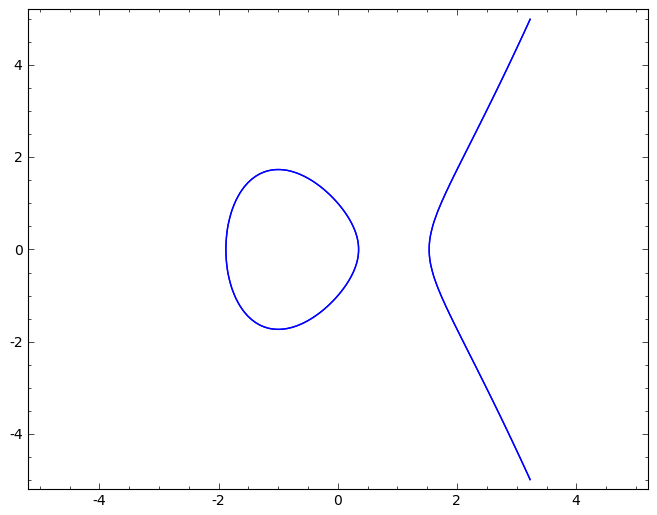
\includegraphics[width=0.5\linewidth]{imagenes/curvaeliptica}
\end{center}
\caption{Curva elíptica $y^2=x^3-3x+1$.}
\label{fig:curvaeliptica}
\end{figure}

%%%%%%%%%%%%%%%%%%%%%%%%%%%%%%%%%%%%%%%%%%%%%%%%%%%
\section{Cálculo de puntos del infinito}
\subsection{Representación homogénea de puntos}
En coordenadas homogéneas todo punto bidimensional está definido por tres coordenadas, de tal modo que un punto con coordenadas $(x, y)$ se representa por la terna: $(X/Z, Y/Z, Z)$. Son útiles en geometría proyectiva porque permiten representar puntos en el infinito.

Otras propiedades que tienen estas coordenadas son:
\begin{enumerate}
\item El punto que representa no cambia si se multiplican las coordenadas por un factor común. Por tanto, dos puntos son iguales si uno se obtiene multiplicando el otro por un factor.
\item Si $Z\neq0 \Rightarrow$ el punto representado $(X/Z, Y/Z)$ está en el plano Euclídeo.
\item Si $Z=0\Rightarrow$ el punto representado es un punto en el infinito.
\item El origen se representa como $O=(0,0,1)$.
\item La terna $(0,0,0)$ no tiene sentido y no representa a ningún punto.
\end{enumerate}

\subsection{Puntos del infinito}

Visualmente podemos entender un punto en el infinito $(a,b,0)$ como un vector con dirección $(a,b)$.

En la figura \ref{fig:puntoinfinito} se puede ver un ejemplo de representación de un punto infinito de coordenadas homogéneas $(2,1,0)$. Este punto es quivalente al $(4,2,0)$, por ejemplo.

\begin{figure}
\begin{center}
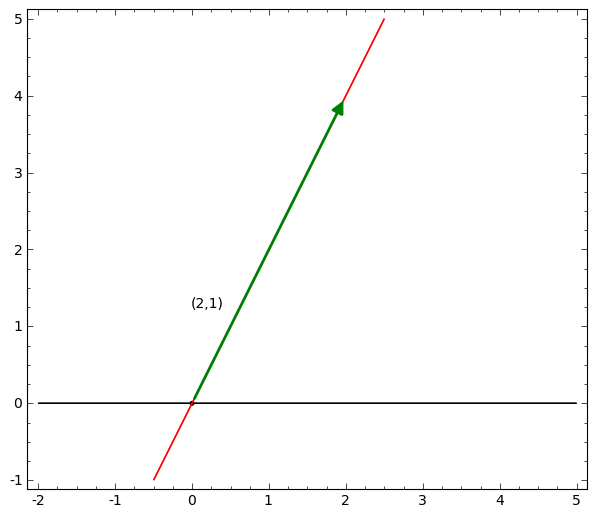
\includegraphics[width=.5\linewidth]{imagenes/puntoinfinito}
\end{center}
\caption{Punto en el infinito con coordenadas $(2,1,0)$.}
\label{fig:puntoinfinito}
\end{figure}

\subsection{Suma de puntos en curvas elípticas}

Se define la suma de dos puntos de la curva elíptica de la siguiente manera. Sean los puntos en coordenadas homogéneas

$$p=(x_1,y_1)$$ $$ q=(x_2,y_2)$$ 
Entonces la suma de $p$ y $q$ es $ p+q=(x_3,y_3)$ donde: $$ x_3=-x_1-x_2+m^2 $$ $$ y_3=-y_1+m(x_1-x_3) $$

$$ m=
\left\{
	\begin{array}{ll}
		\frac{y_1-y_2}{x_1-x_2}  & \mbox{si } x_1\neq x_2,y_1\neq y_2  \\
		\frac{3x_1^2-3}{2y_1} & \mbox{si }  x_1=x_2,y_1=y_2
	\end{array}
\right.
$$

Por ejemplo, sea la curva elíptica $x^3-3x+1-y^2$ y dos puntos $p=(0,1)$ y $q=(-1,\sqrt{3})$ pertenecientes a la curva (ver figura \ref{fig:sumapuntos}).

\begin{figure}[h]
\begin{center}
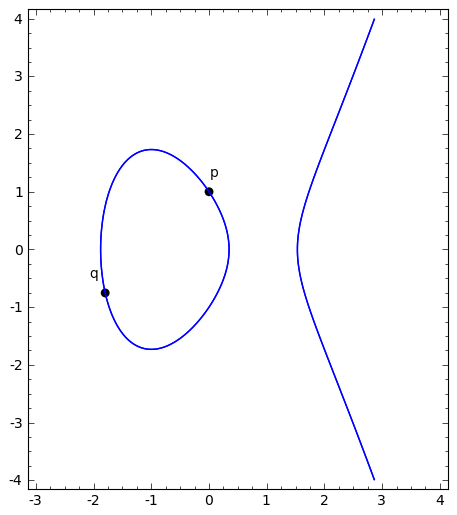
\includegraphics[width=.5\linewidth]{imagenes/sumapuntos}
\end{center}
\caption{Curva elíptica con un punto $p=(0,1)$ y $q=(-1,\sqrt{3})$.}
\label{fig:sumapuntos}
\end{figure}

Para hallar la suma gráficamente hay que trazar la recta secante que une a los puntos $p$ y $q$.

%%%%%%%%%%%%%%%%%%%%%%%%%%%%%%%%%%%%%%%%%%%%%%%%%%%
\section{Aplicación en criptografía}

\bibliographystyle{plain}
\bibliography{refs} % mi archivo refs.bib
\end{document}
